\section{Background and related work}\label{sec:background}

\subsection{Valency and valency phenomena}\label{subsec:valency}

% valency - terminology introduction

In chemistry, \textit{valency}, or \textit{valence}, refers to the combining power of an atom or radical. The valency of any atom can be measured by the number of hydrogen atoms that it can combine with or displace in a chemical compound \citep{law2020a}. This same term has been used in linguistics to similar effect and refers to the combining power of a word, primarily a verb or other predicate, with other words or elements of the sentence. 

Lucien Tesnière is generally credited with introducing the term valency to linguistics with his syntactic theory of valency and dependence, as presented in the posthumously published \textit{Éléments de syntaxe structurale} (\cite*{tesniere1959}; English translation \cite*{tesniere2015}).\footnote{
    It should be noted that while Tesnière is rightly credited with the introduction of a theory of linguistic valency, the metaphor of valency itself has made appearances as early as in \citet{peirce1897}, among others \citep{przepiorkowski2018}.
}
In another of Tesnière's metaphors, each verbal node, being the center of sentence structure, is not unlike a ``theatrical performance'' with the verb expressing the process and the nouns being the \textit{actants} (what we would now call \textit{arguments}) in this performance. Just like how atoms of different elements allow for a greater or lesser number of bonds, different verbs can combine with a greater or lesser number of actants, i.e., their valency.

% the phenomena now we are now calling valency - different theories
While the term valency is borrowed into linguistics from chemistry, the study of the phenomena which are covered by or otherwise overlap with valency has a much longer tradition, dating to the early beginnings of linguistics from the kāraka concept of semantic relation between verb and noun \citep{ganeri2011a} in Pāṇinian grammar to modern case grammar \citep{fillmore1968}. 

Most linguistic theories assert the centrality of the verb in determining either or both the syntactic and semantic structure of a sentence, corroborated also by psycholinguistic evidence \citep{healy1970}. This places valency and the issues of \textit{argument structure} squarely at the center of the inquiry into the interface between lexical semantics and syntax.

%% subcategorization in generative grammar
In generative grammar, the syntactic valency of a verb is treated under a similar notion of \textit{subcategorization} \citep{chomsky1965a}. As an example, a transitive verb must be followed by a direct object, whereas an intransitive verb cannot. As such, transitive and intransitive verbs form subcategories of the verb category. Verbs are therefore assigned to \textit{subcategorization frames} which specify the number and type of complements, i.e., objects and obliques, as well as of the subject in later theories, that the verb can be subcategorized for. In addition to being syntactically driven, a notable feature of generative theories' treatment of valency is that the subcategorization frames are considered as part of the lexical entry of the verb. Later work in generative grammar, in particular \citet{jackendoff1972,jackendoff1987,jackendoff1992}, following \citet{katz1963} and \citet{gruber1962}, further developed a theory of thematic relations and posited that argument structure serves as the interface between syntactic and thematic structures.
% unclear on relationship between subcategorization and selection in generative grammar; also maybe more citations and examples here later
%% Levin
As compared to broader distinctions such as those made between transitive and intransitive verbs, \citet{levin1993} provided a much more fine-grained categorization of verbs into different verb classes based on their syntactic behavior. Building on the assumption that the syntactic behavior of verbs are determined semantically, Levin reasons that patterning together classes of verbs based on their diathesis alternations should result in semantically coherent verb classes. Levin's work has been highly influential both in the development of valency theory and in computational approaches to lexical semantics, the VerbNet \citep{kipper-schuler2005, kipper2006, kipper2008} being a prominent example of such projects, extending the Levin verb classes into a computational lexicon that links with other resources such as WordNet \citep{fellbaum1998, miller1995}, PropBank \citep{kingsbury2002} and FrameNet \citep{baker1998, fillmore2015}.

%% frame semantics - fillmore
In terms of their theoretical foundations, however, FrameNet differs from VerbNet in that it derives from a different line of research that stems from Charles Fillmore's frame semantics \citep{fillmore1977, fillmore1977a, fillmore1982}, which in turn traces to his earlier work on case grammar \citep{fillmore1968,fillmore1970}. While they are computationally interoperable to some extent, there remains a key conceptual distinction made in frame semantics \citet{fillmore1968}, namely the \textit{frames}-driven analysis of argument encoding. While the verbal lexicon continues to play a role in placing selectional restrictions on the frames in which a given verb can be found in, the frames are themselves said to have semantics through their grouping of frame elements, which are similar to thematic roles but local to their specific frames. The frame semantics approach is consolidated by further development in construction grammar where the frames viewed as constructions, namely \textit{argument structure constructions} \citep{goldberg1992,goldberg1995}. Furthermore, construction grammar theories often advocate for frames being considered distinct or autonomous constructions, as it is not strictly predictable from other constructions.

\todo{q: I am still considering how the conceptual distinction of valency information as part of the lexical entry of the verb vs. valency information as part of a frame construction affects their predictions in terms of typological evidence. Would, say, a hypothetical result where cross-lingual patterns in the organization of verbal lexicon can be observed, but the frames themselves are more language-specific, necessarily be evidence against frame as a distinct / autonomous construction? need to think more about frame semantics and typology}

% \subsection{Dependency grammars}\label{subsec:depgrammar}
\subsection{Typological perspectives on valency and dependency}\label{subsec:typology}

It is perhaps not surprising that, besides introducing the first theory of linguistic valency, \citet{tesniere1959} also introduced the notion of dependency into modern linguistics.

In terms of their mathematical foundations, dependency grammar, based on the notion of dependencies, can be viewed in contrast with constituency grammars which are based on the notion of substitution instead\citep{stabler2019}. However, even most iterations of generative grammar theories, which are primarily constituency-based, incorporate some notion of a head-dependent relationship (cf. X-bar theory). \citet{demarneffe2019} cites the easiness of generalization across languages, its operationalization of human sentence processing facts, and the transparency and simplicity of representation as reasons why dependency-based representations have become increasingly widely adopted in linguistic theory and even more so in NLP.

Already \citet{tesniere1959} paid attention to the cross-lingual differences in the argument structure of semantically equivalent sentences. Tesnière described the process of \textit{metataxis}, by which syntactic structures of one language is ``translated'' to those of another. This implies, as this study argues explicitly, that the primary typological interest in valency is in comparing the mismatches. The usefulness of dependency grammar in allowing for cross-lingual generalizations and comparisons should not be understated. 

\todo{intro UD}

\begin{figure}
    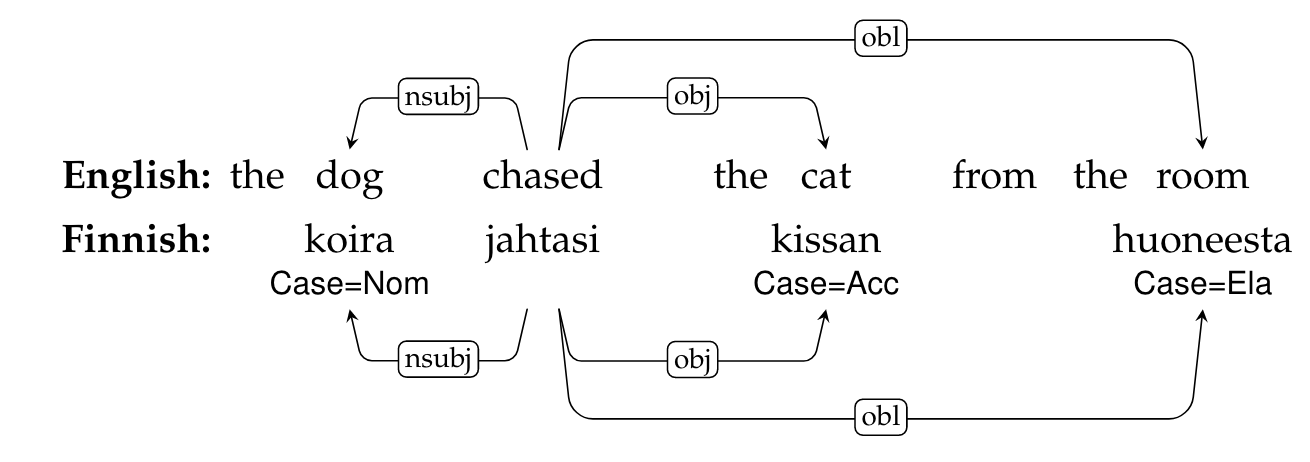
\includegraphics[width=0.85\textwidth]{figures/ud_example_sentence.png}
    \centering
    \caption{Simplified UD annotation for equivalent sentences from English (top) and Finnish (bottom) \citep{demarneffe2021}.}\label{fig:ud-example-sentence}
\end{figure}
 
\todo{a few words on cross-lingual contrastive studies}


What would a universal look like? \citet{tsunoda1981, tsunoda1985, tsunoda2015} proposes a hierarchy of verbs.

Frame based approach: \citet{baker2020, ellsworth2021} addresses FrameNet and typology; in contrast, \citet{say2014} rejects the equating of minor valency classes cross-lingually and study how the individual verbs are grouped.

% why approach valency from typological perspective

% cross-lingual contrastive studies
% Cross-lingual contrastive studies are, generally bilingual and mostly between English and German. 

% \citet{levin2005} identify five major questions that are necessary for a complete theory of argument realization.
% \todo{copy from hand notes and add how a typological study relates some of these questions}

% other typological approaches

% With computational work: one of the key issue to pay attention to is whether the valency frames / verb classes are syntactically or semantically derived. Important to be clear to avoid circularity and since we're dealing with syntax-semantics interface.

\citet{croft2017} address UD specifically and propose more typologically-informed modifications to the dependency annotations of UD. 

Computational work on semantic frame induction / verb classes:  \citet{abend2009, basili1993, bickel2014, dowty1991, fellbaum1998, fillmore1968, furstenau2012, kipper-schuler2005, kipper2008, korhonen2006, levin2015, majewska2018, majewska2020, majewska2021, miller1990, miller1995, navarretta2000, palmer2005, say2014, sayeed2018, schulteimwalde2002, schulteimwalde2003, schulteimwalde2006, snider2006, sun2008, sun2009, sun2013, titov2012, watanabe2010, yamada2021} 
\todo{pick a few examples to introduce, e.g., one each for semantics- and synatx-based approaches and omit the rest / relegate to citations only}




